% -*- coding: utf-8 -*-
\documentclass[8pt]{beamer}
\newcounter{myframenumber}
\usepackage{amsfonts,amsmath,oldgerm}
\usepackage{booktabs}
\usepackage{multirow}
\usepackage{capt-of}
\usepackage{float}
\usepackage{hyperref}           % <-- UNA sola volta
\usepackage{tikz}
\usetikzlibrary{arrows.meta}
\usepackage{media9}
\usepackage{multimedia}

\usepackage{tikz}
\usetikzlibrary{positioning}
\usetikzlibrary{arrows.meta}


\usepackage[absolute,overlay]{textpos}
\usepackage{graphicx}

\usetheme{sintef}
\usefonttheme[onlymath]{serif}

\setbeamerfont{frametitle}{size=\large}
\setbeamerfont{normal text}{size=\tiny}
\setbeamerfont{title}{size=\Huge}
\setbeamerfont{subtitle}{size=\large}
\setbeamerfont{course}{size=\normalsize}
\setbeamerfont{author}{size=\normalsize}

\newcommand{\testcolor}[1]{\colorbox{#1}{\textcolor{#1}{test}}~\texttt{#1}}
\newcommand{\hrefcol}[2]{\textcolor{cyan}{\href{#1}{#2}}}

\title{{DNA Methylation Analysis: Statistics and Machine Learning in Breast Cancer}}
\subtitle{Thesis Work Presentation}
\course{Master's Degree in Mathematical Engineering}
\author{Elisabetta Roviera}
\titlebackground*{assets/background}

\begin{document}

\begin{frame}
    \titlepage
    \begin{textblock*}{5cm}(10.5cm,2.5cm) % ↓ abbassato da 2.2cm a 1.75cm
        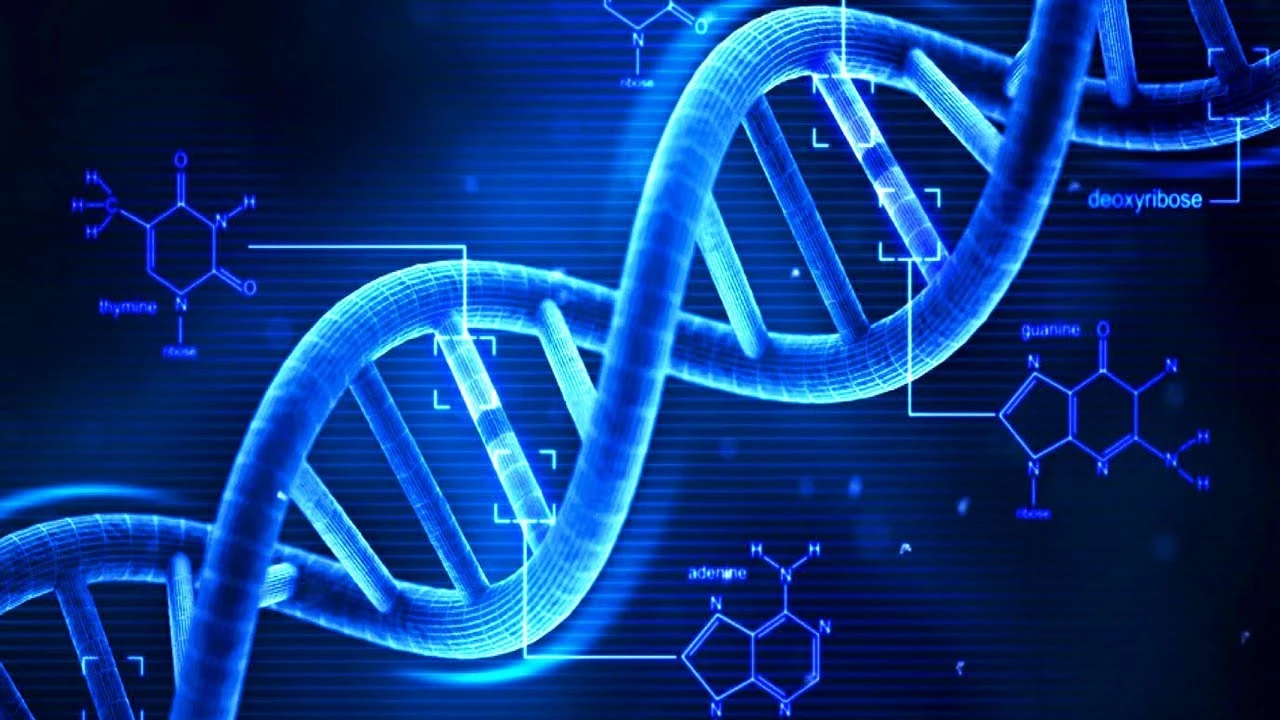
\includegraphics[width=5cm,keepaspectratio]{slide1.png}
    \end{textblock*}
\end{frame}

\begin{frame}{Introduction: Goals of the Presentation}
    \begin{itemize}
        \item My background: Mathematical Engineering and Data Science
        \item Objective: show how quantitative tools can be applied to biomedical problems
        \item Case study: DNA methylation in breast cancer
    \end{itemize}
\end{frame}

\begin{frame}{Breast Cancer: Context and Relevance}
    \begin{itemize}
        \item High incidence worldwide
        \item Importance of early detection for patient outcomes
        \item Why data matters: quantitative analysis supports screening, diagnosis, and risk assessment
    \end{itemize}

    \vspace{0.4cm}
    \centering
    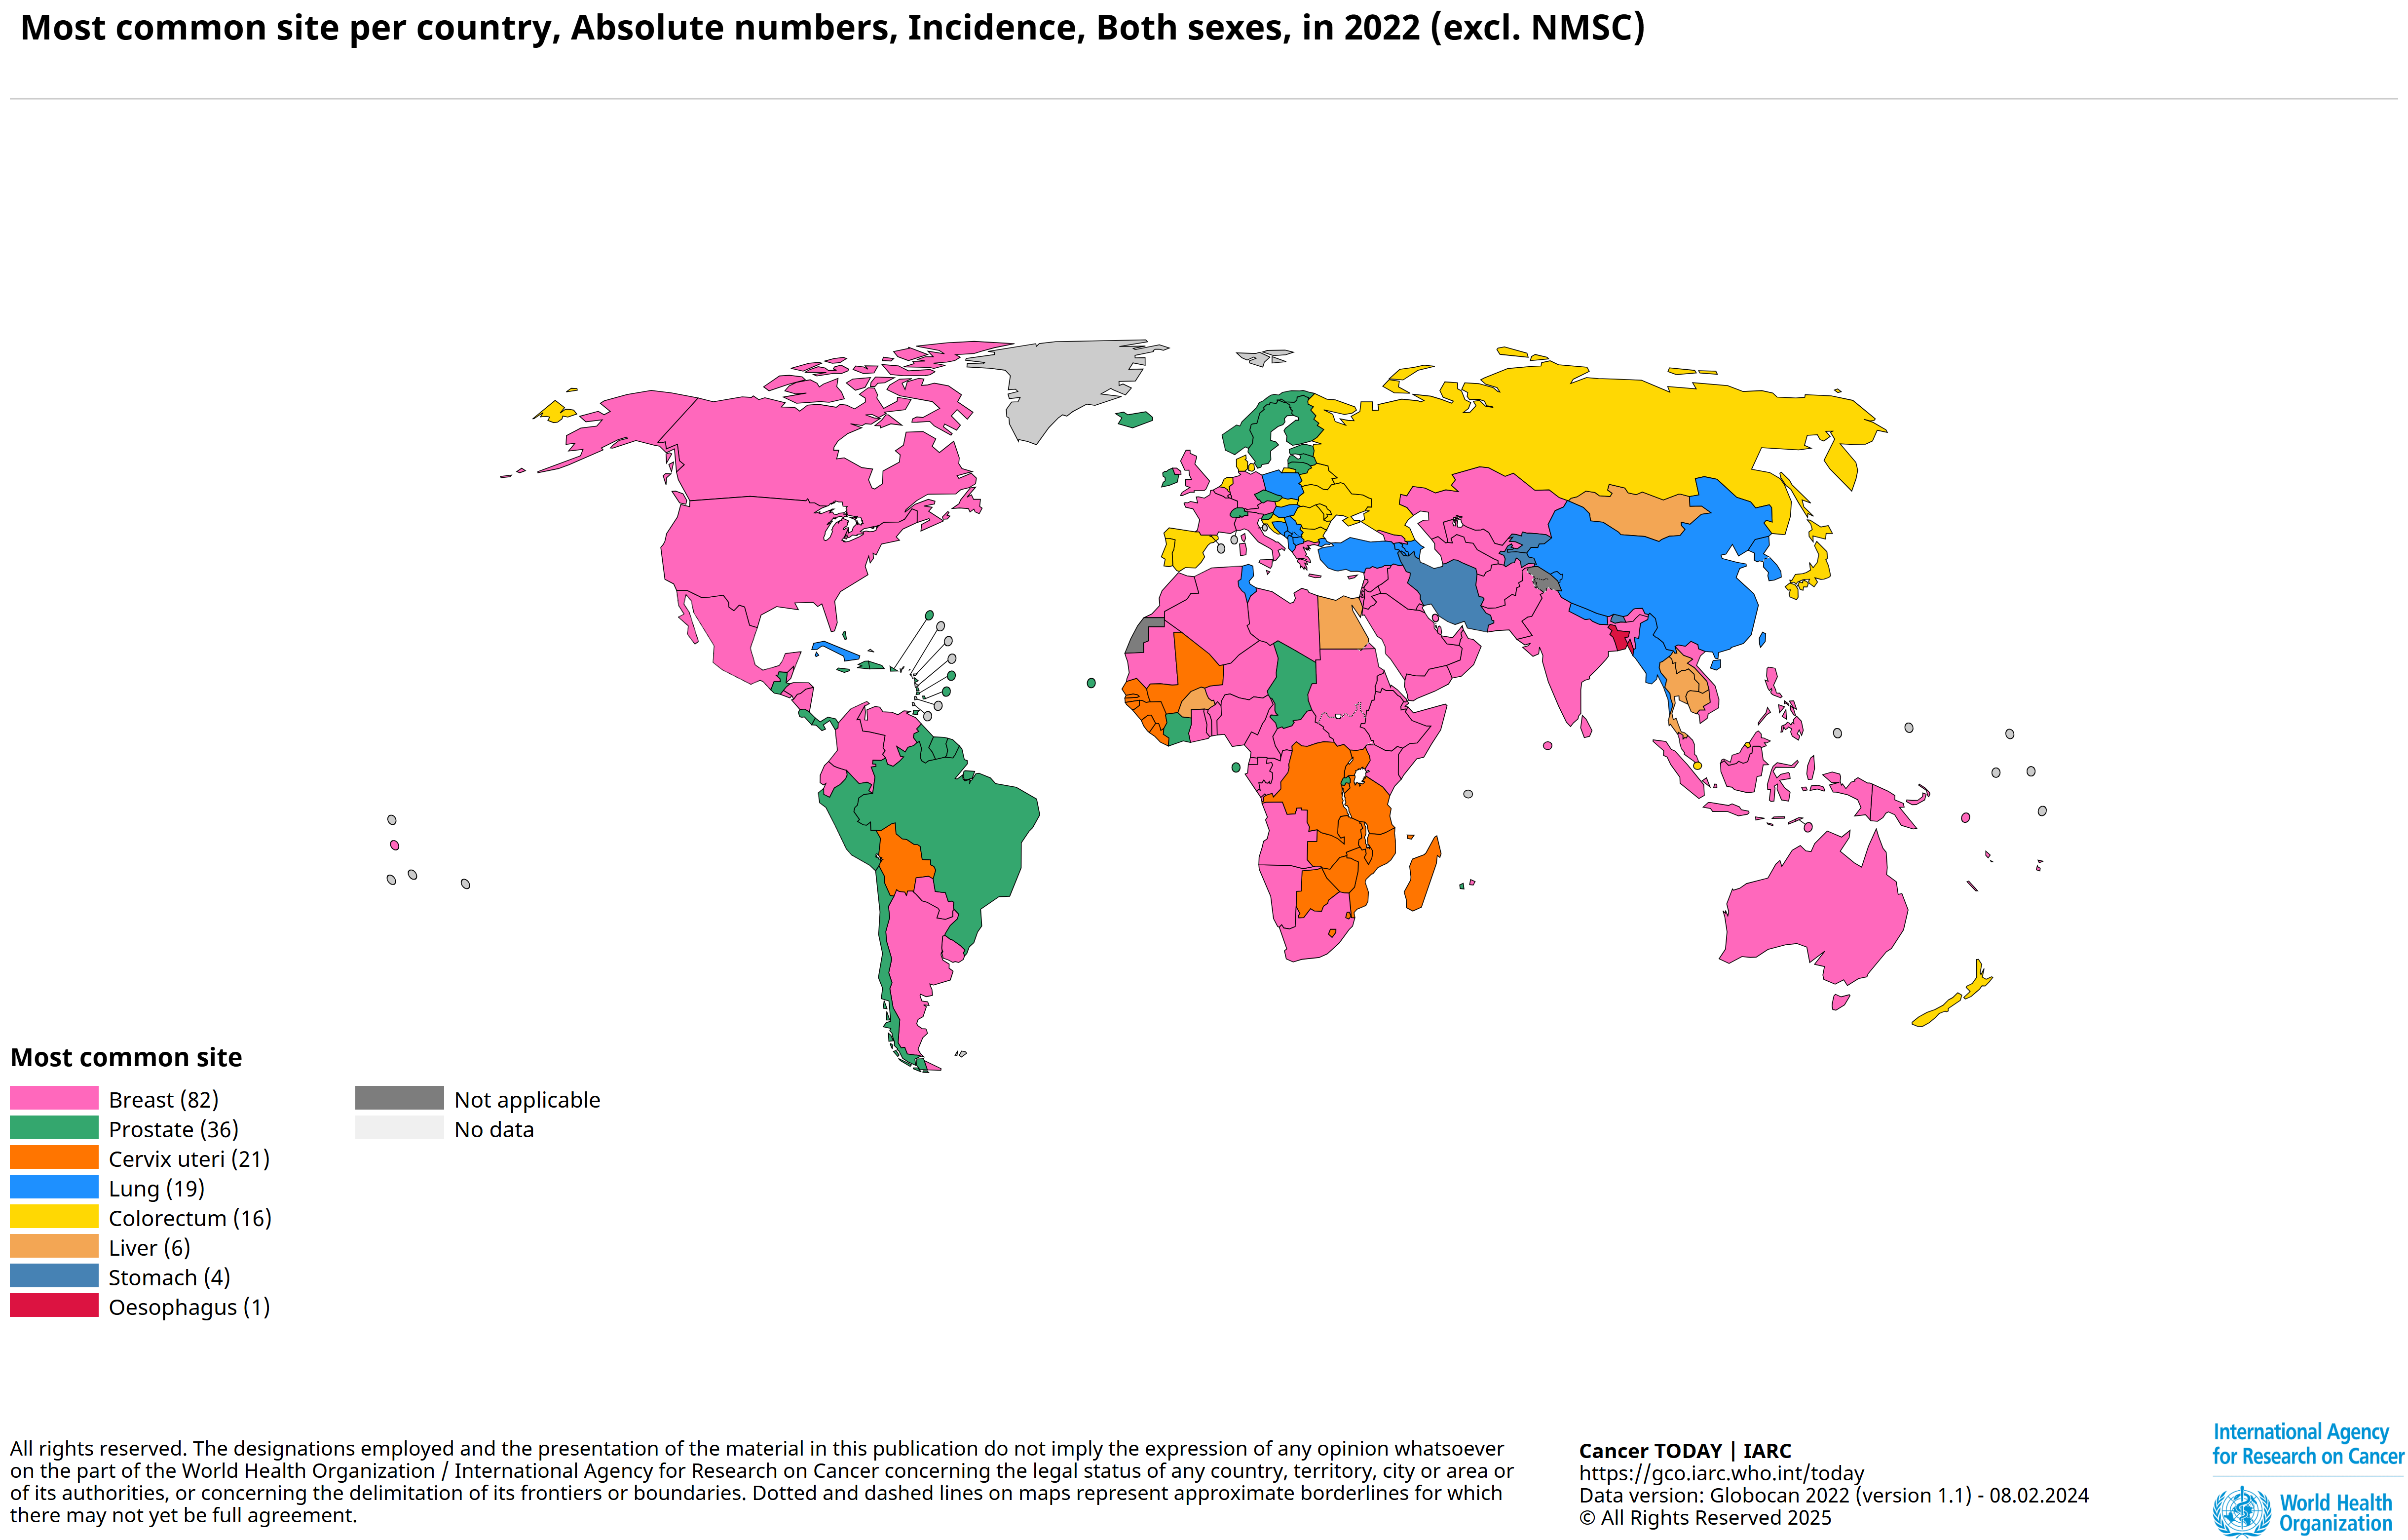
\includegraphics[width=0.65\textwidth]{slide3.png} % replace with actual figure
\end{frame}

\begin{frame}{CpG and $\beta$-values: The Language of Epigenetic Data}
    \begin{itemize}
        \item CpG sites: genomic positions where DNA methylation can occur
        \item $\beta$-value $\in [0,1]$: proportion of methylation at each CpG
        \item Methylation modulates gene regulation
        \item In cancer: both hypermethylation and hypomethylation emerge
    \end{itemize}

    \vspace{0.4cm}
    \centering
    % Replace with your density plot
    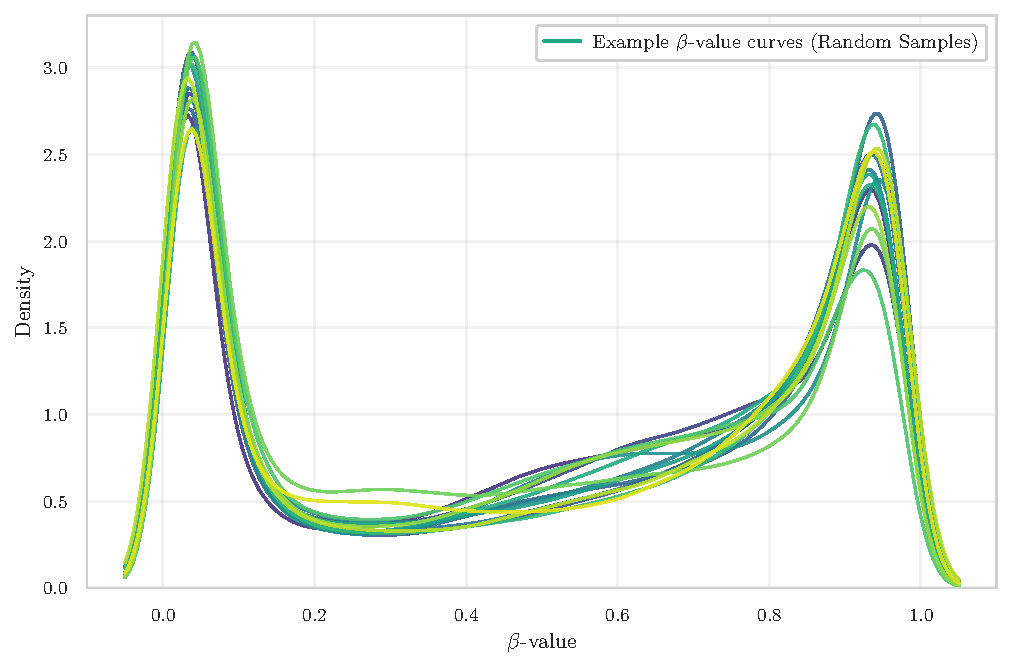
\includegraphics[width=0.70\textwidth]{slide4.pdf}
\end{frame}

\begin{frame}{Field Cancerization: The Central Research Question}
    \begin{itemize}
        \item Is “normal” tissue near the tumor already epigenetically altered?
        \item As Dr.\ Gambino highlights: \\
              \emph{“Identify early methylation alterations in normal tissues and assess their role in tumor initiation.”}
        \item Concept of field cancerization
    \end{itemize}

    \vspace{0.4cm}
    \centering

    \begin{columns}[c]
        \column{0.48\textwidth}
            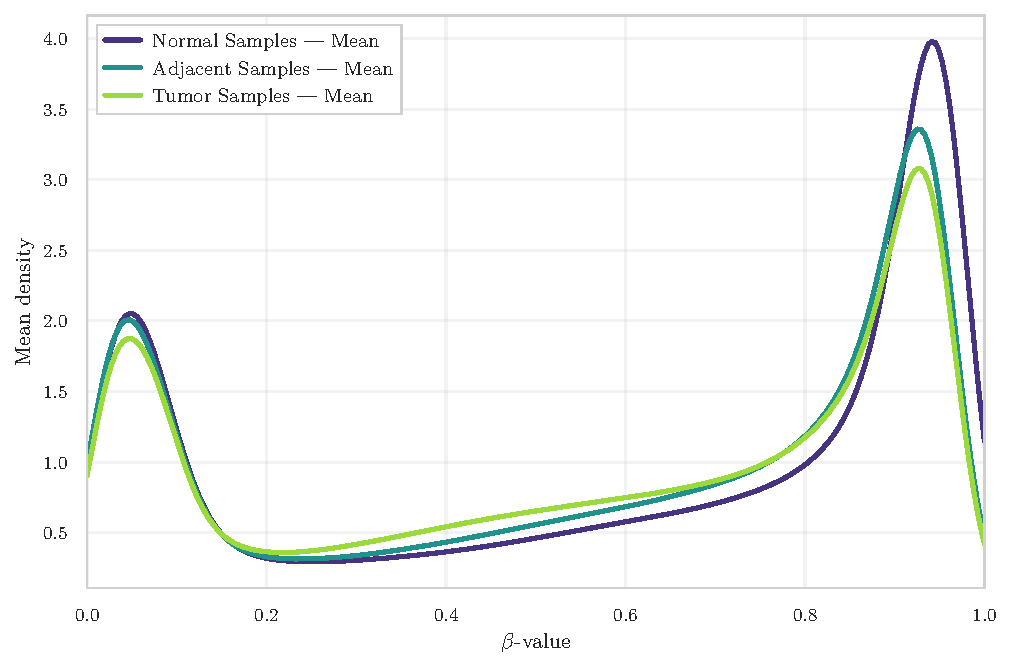
\includegraphics[width=\textwidth]{slide5_a.pdf}

        \column{0.48\textwidth}
            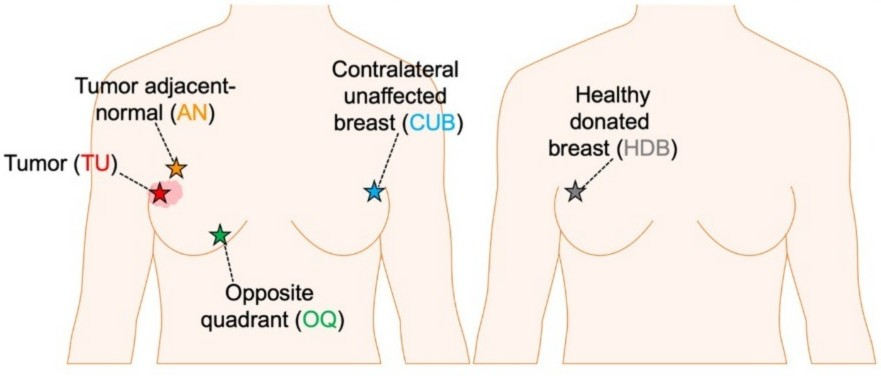
\includegraphics[width=\textwidth]{slide5_b.jpeg}
    \end{columns}
\end{frame}


\begin{frame}{Field Cancerization: The Central Research Question}
    \begin{itemize}
        \item Is “normal” tissue near the tumor already epigenetically altered?
        \item As Dr.\ Gambino highlights: \\
              \emph{“Identify early methylation alterations in normal tissues and assess their role in tumor initiation.”}
        \item Concept of field cancerization
    \end{itemize}

    \vspace{0.4cm}
    \centering

    \begin{figure}
        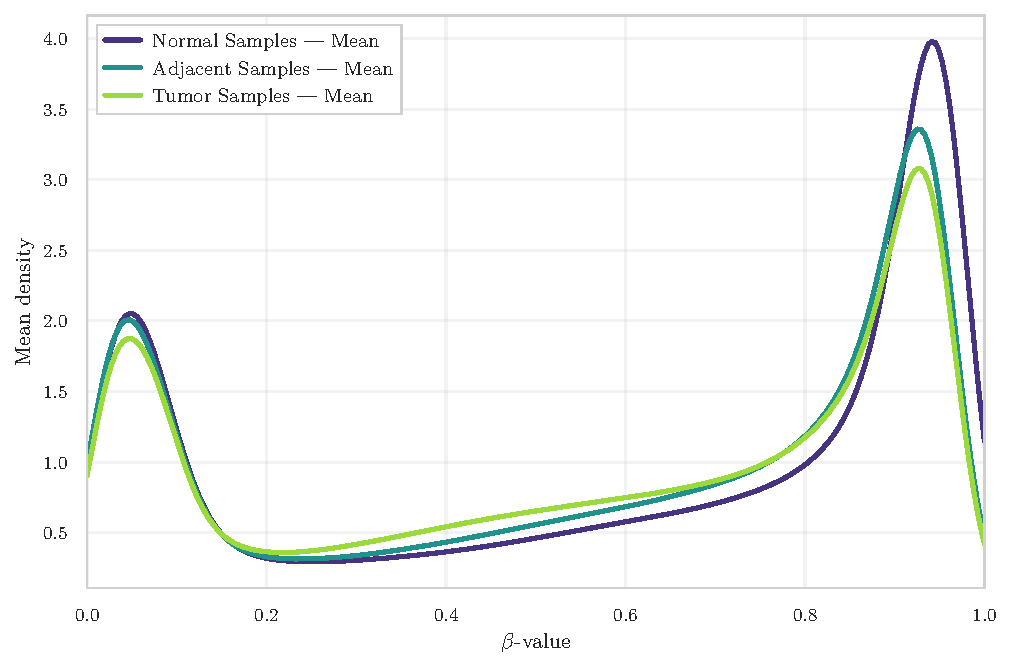
\includegraphics[width=0.48\textwidth]{slide5_a.pdf}
        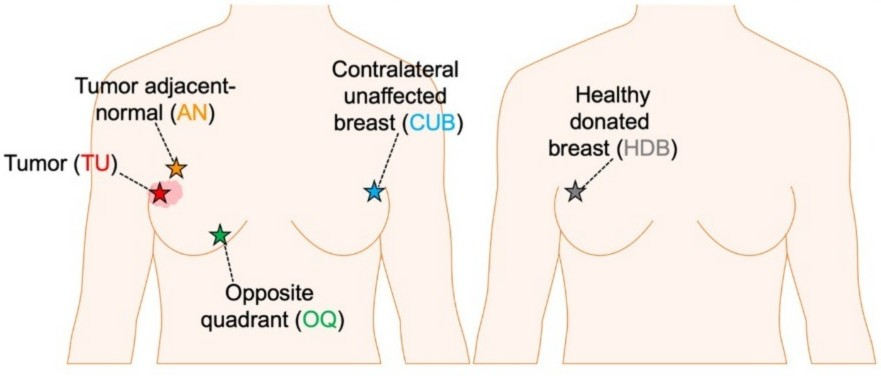
\includegraphics[width=0.48\textwidth]{slide5_b.jpeg}
    \end{figure}

\end{frame}

\begin{frame}{Accessing and Understanding the Data}
    \begin{itemize}
        \item GEO datasets: heterogeneous formats and incomplete metadata
        \item Small $n$, huge $p$ (up to 800k CpG sites)
        \item Raw IDAT files vs.\ preprocessed $\beta$-value matrices
        \item Unknown or inconsistent preprocessing in some datasets
    \end{itemize}

    \vspace{0.4cm}
    \centering
    \begin{tabular}{lcc}
        \toprule
        \textbf{Dataset} & \textbf{Samples ($n$)} & \textbf{CpGs ($p$)} \\
        \midrule
        GSE69914   & 397 & 485{,}512 \\
        GSE225845  & 477 & 750{,}426 \\
        GSE287331  & 311 & 702{,}573 \\
        \bottomrule
    \end{tabular}
\end{frame}

\begin{frame}{Computational Challenges}
    \begin{itemize}
        \item Huge files → use of Parquet format, LZ4 compression, chunked loading
        \item Strict RAM constraints on Kaggle environments
        \item Need for Illumina manifest alignment to correctly map probe IDs
    \end{itemize}

    \vspace{0.6cm}
    \centering

    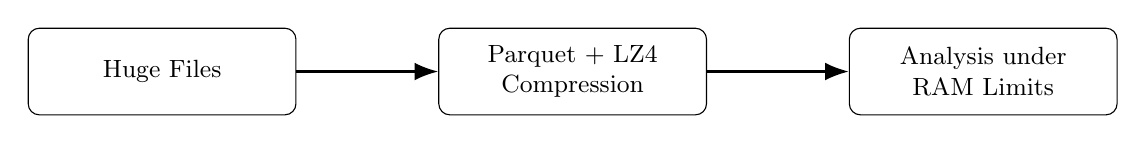
\begin{tikzpicture}[
        node distance=1.8cm,
        box/.style={
            rectangle,
            draw,
            rounded corners,
            minimum width=3.4cm,
            minimum height=1.1cm,
            align=center,
            font=\small
        },
        arrow/.style={
            -{Latex[length=3mm]},
            thick
        }
    ]

    % Nodes
    \node[box] (bigfiles) {Huge Files};
    \node[box, right=of bigfiles] (parquet) {Parquet + LZ4\\Compression};
    \node[box, right=of parquet] (ram) {Analysis under\\RAM Limits};

    % Arrows
    \draw[arrow] (bigfiles) -- (parquet);
    \draw[arrow] (parquet) -- (ram);

    \end{tikzpicture}

\end{frame}


\begin{frame}{Can We Merge the Datasets?}
    \begin{itemize}
        \item Different array platforms (HM450 vs.\ EPIC)
        \item Heterogeneous and partly unknown preprocessing pipelines
        \item Direct merge would introduce strong batch and platform effects
        \item Decision: perform all analyses within each dataset (intra-dataset)
    \end{itemize}

    \vspace{0.5cm}
    \centering

    \begin{columns}[c]
        \column{0.48\textwidth}
            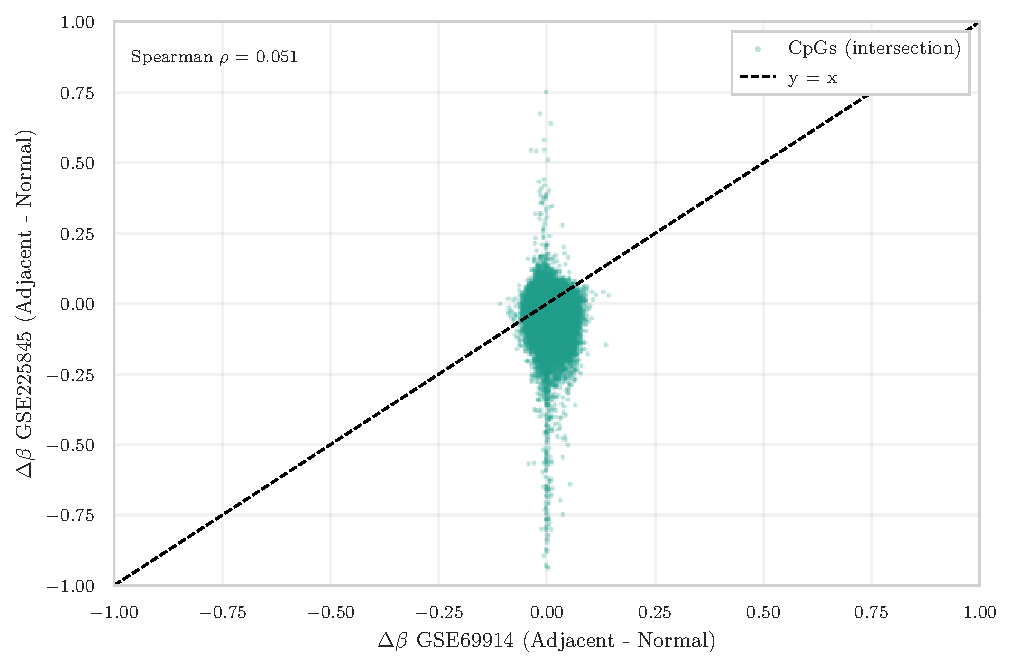
\includegraphics[width=\textwidth]{slide8_a.pdf}

        \column{0.48\textwidth}
            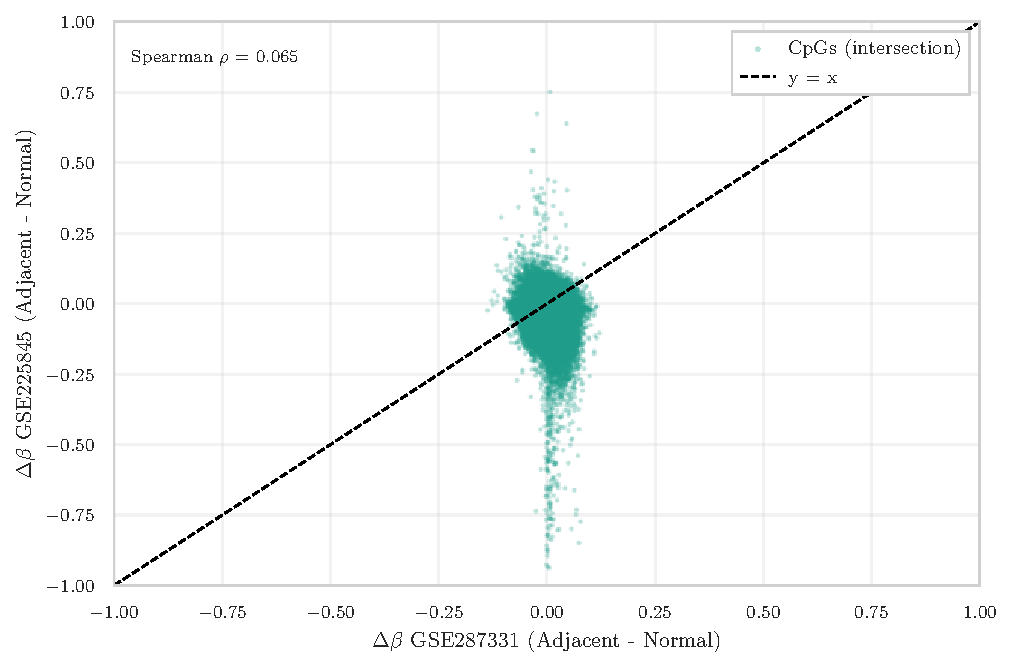
\includegraphics[width=\textwidth]{slide8_b.pdf}
    \end{columns}
\end{frame}


\begin{frame}{Global DNA Methylation Distributions}
    \begin{itemize}
        \item Canonical bimodal $\beta$-value distribution (unmethylated vs.\ highly methylated CpGs)
        \item Tumor samples: shift towards hypomethylation and increased heterogeneity
        \item Adjacent samples: early, subtle deviations from the Normal baseline
    \end{itemize}

    \vspace{0.4cm}
    \centering
    % Replace with your boxplot of global methylation summaries
    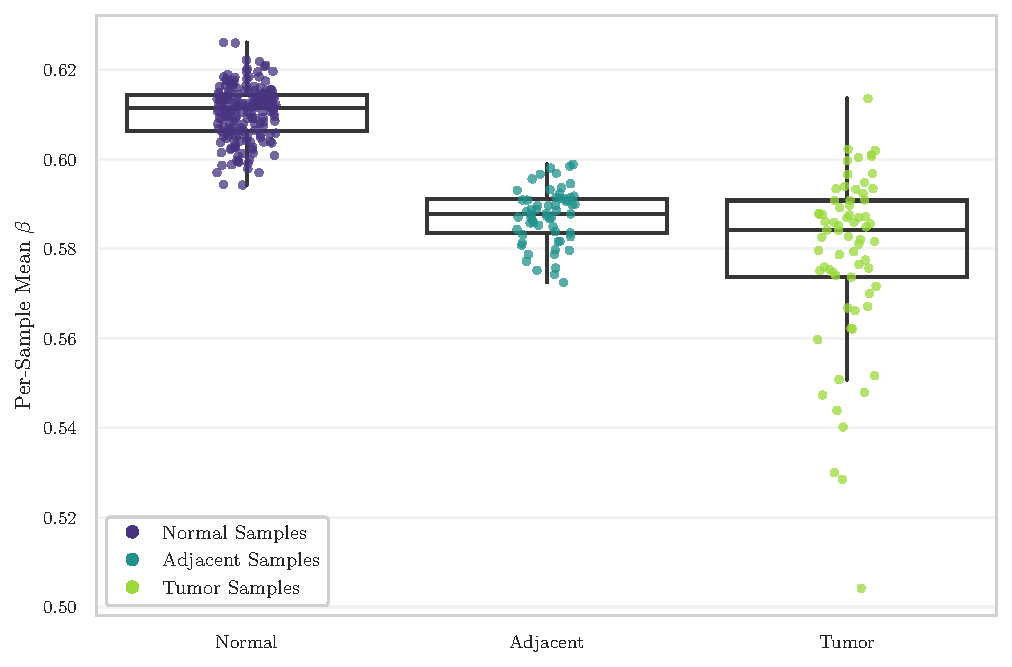
\includegraphics[width=0.75\textwidth]{slide9.pdf}
\end{frame}

\begin{frame}{Variability and Epigenetic Outliers}
    \begin{itemize}
        \item Tumor samples show higher methylation variability
        \item Adjacent tissue exhibits more focal, localized signals
        \item Highly unstable CpGs are promising biomarker candidates
    \end{itemize}

    \vspace{0.4cm}
    \centering
    % Heatmap of top outlier CpGs (e.g., per dataset or example dataset)
    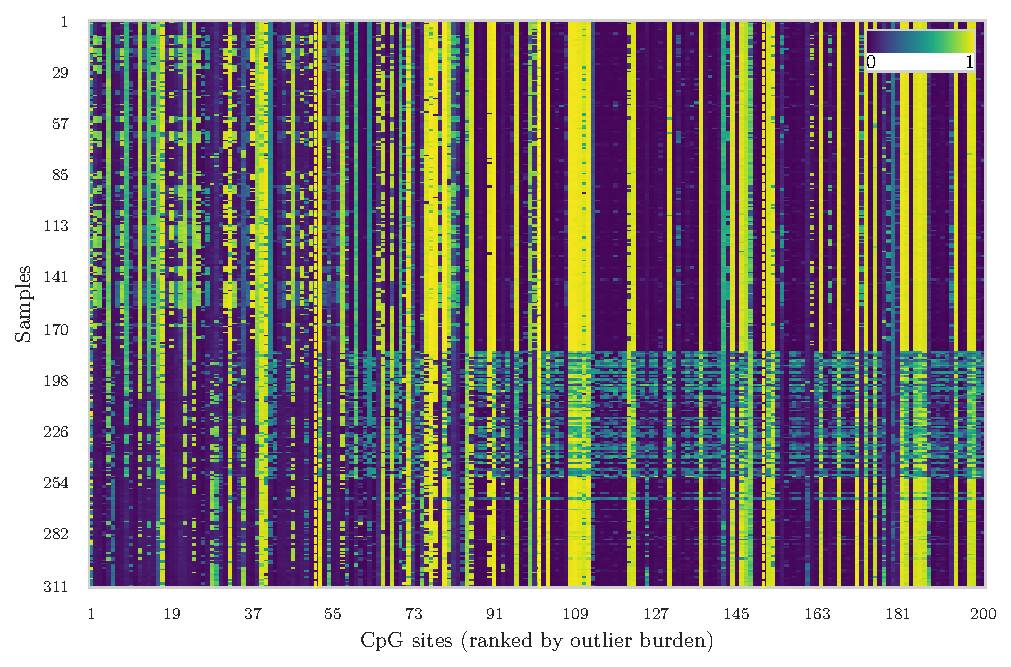
\includegraphics[width=0.75\textwidth]{slide10.pdf}
\end{frame}

\begin{frame}{Dataset Embeddings and Group Structure}
    \begin{itemize}
        \item GSE69914: strong overlap between groups
        \item GSE225845: more complex, diffuse patterns
        \item GSE287331: clear separation between Normal, Adjacent, and Tumor
    \end{itemize}

    \vspace{0.4cm}
    \centering
    \begin{columns}[c]
        \column{0.48\textwidth}
            \centering
            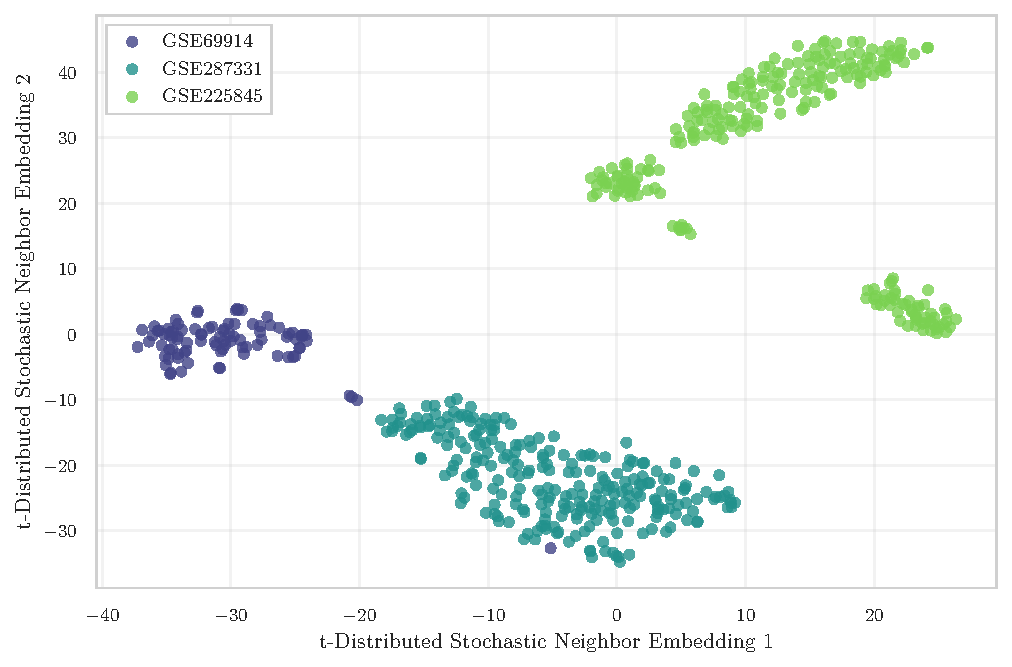
\includegraphics[width=\textwidth]{slide11_a.pdf}\\
            \scriptsize t-SNE coloured by tissue state

        \column{0.48\textwidth}
            \centering
            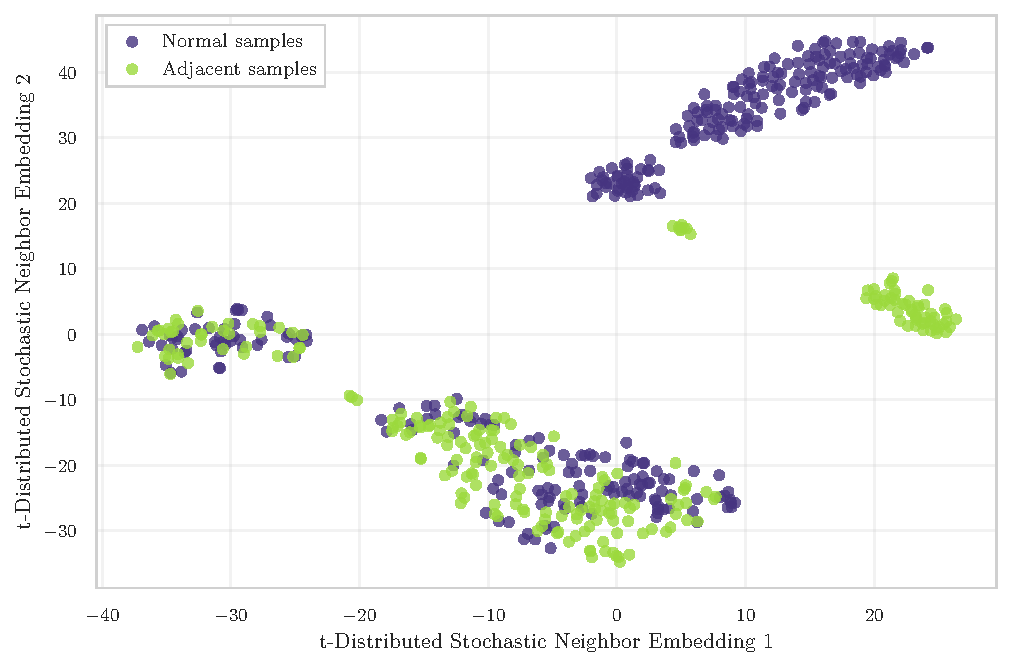
\includegraphics[width=\textwidth]{slide11_b.pdf}\\
            \scriptsize t-SNE coloured by dataset
    \end{columns}
\end{frame}

\begin{frame}{Probe-Design Bias and BMIQ Normalization}
    \begin{itemize}
        \item Two probe designs (Type I vs.\ Type II) with incompatible $\beta$-distributions
        \item Real case: GSE287331 shows a strong uncorrected probe-design bias
        \item BMIQ performs quantile mapping of Type II probes toward the Type I distribution
        \item Caveat: BMIQ can reduce biological variability and partially mask real signals
    \end{itemize}

    \vspace{0.4cm}
    \centering
    \begin{columns}[c]
        \column{0.48\textwidth}
            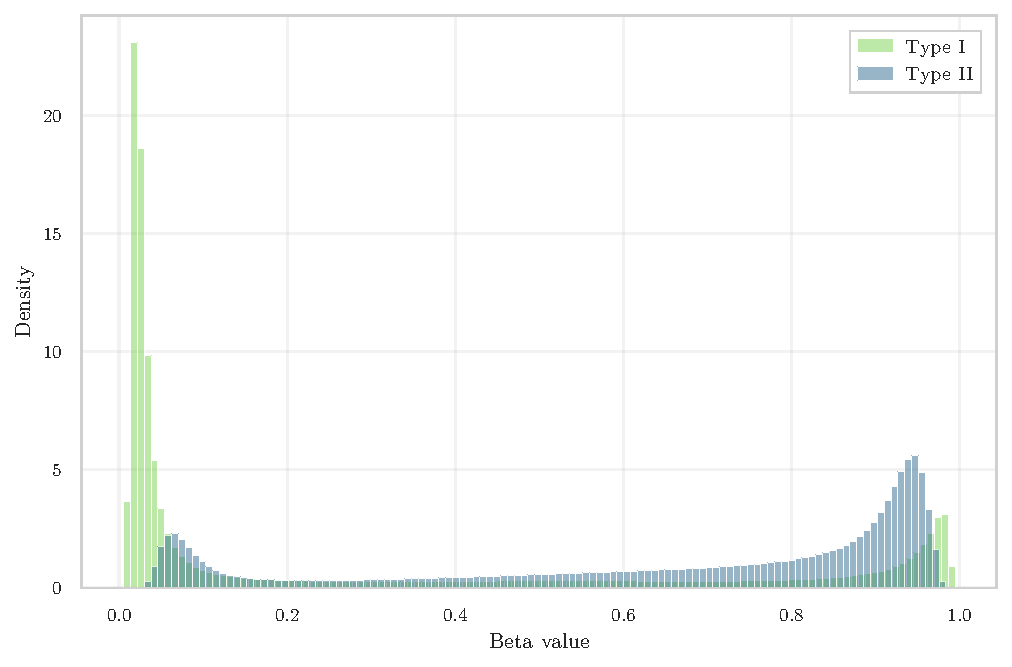
\includegraphics[width=\textwidth]{slide12_a.pdf}\\
            \scriptsize Pre-BMIQ: Type I vs Type II

        \column{0.48\textwidth}
            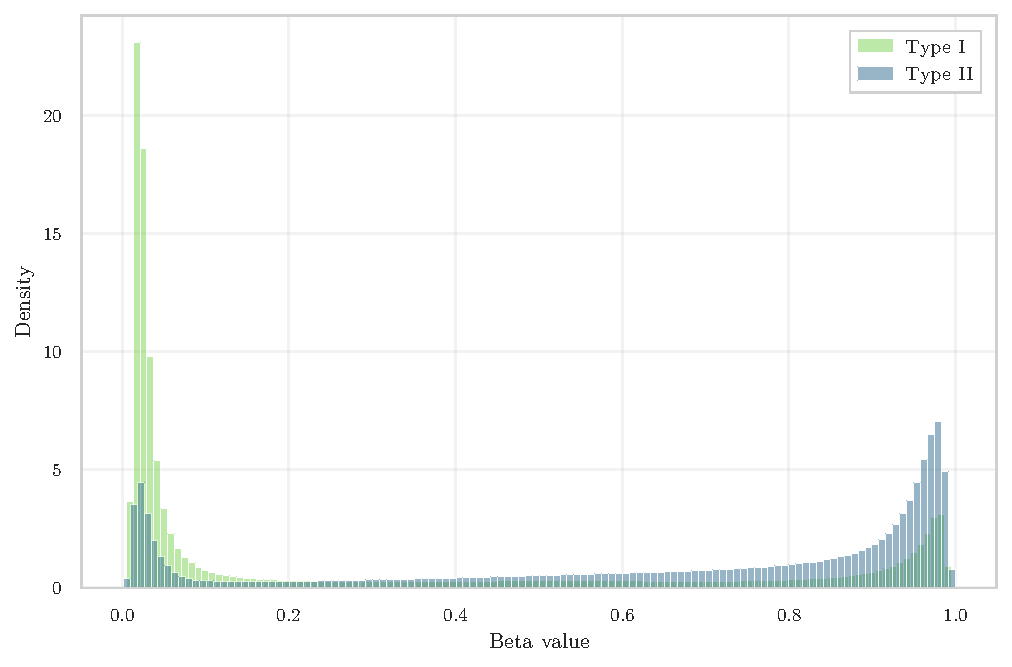
\includegraphics[width=\textwidth]{slide12_b.pdf}\\
            \scriptsize Post-BMIQ: Type I vs Type II
    \end{columns}
\end{frame}

\begin{frame}{Feature Selection in High Dimensions}
    \begin{itemize}
        \item $p \gg n$ → dimensionality reduction and filtering are essential
        \item Technical filters: cross-reactive probes, SNP probes, non-CpG probes, Illumina manifest
        \item Evaluate and correct potential batch effects (e.g., COMBAT)
        \item Three families of feature selection strategies:
        \begin{itemize}
            \item Statistical: $\Delta\beta$, variance filtering, stability measures
            \item Biological: promoters, CpG islands, curated gene sets
            \item ML-based: Lasso, decision trees, embedded model selection
        \end{itemize}
    \end{itemize}

    \vspace{0.4cm}
    \centering

    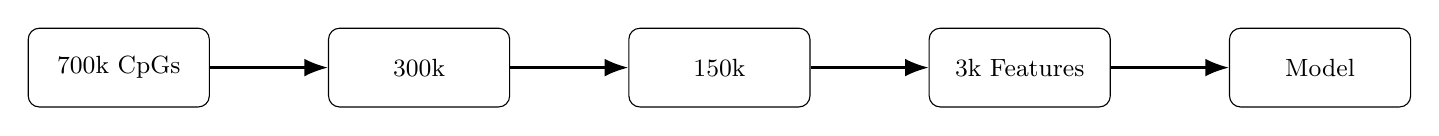
\begin{tikzpicture}[
        box/.style={
            rectangle,
            draw,
            rounded corners,
            minimum width=2.3cm,
            minimum height=1cm,
            align=center,
            font=\small
        },
        arrow/.style={-{Latex[length=3mm]}, thick},
        node distance=1.5cm
    ]

    \node[box] (d1) {700k CpGs};
    \node[box, right=of d1] (d2) {300k};
    \node[box, right=of d2] (d3) {150k};
    \node[box, right=of d3] (d4) {3k Features};
    \node[box, right=of d4] (model) {Model};

    \draw[arrow] (d1) -- (d2);
    \draw[arrow] (d2) -- (d3);
    \draw[arrow] (d3) -- (d4);
    \draw[arrow] (d4) -- (model);

    \end{tikzpicture}

\end{frame}

\begin{frame}{ML in Non-Ideal Conditions}
    \begin{itemize}
        \item Train / validation / test with extremely small $n$
        \item Generalizing across datasets (A $\rightarrow$ B) is often unreliable
        \item How many features to select? Which metrics to use?
        \item Overfitting, noise, limited interpretability
        \item Deep Learning: training from scratch is infeasible $\rightarrow$ only pre-trained / transfer learning methods
    \end{itemize}

    \vspace{0.45cm}
    \centering
    \begin{tabular}{lcccc}
        \toprule
        \textbf{Approach} & \textbf{Data Need} & \textbf{Interpretability} & \textbf{Robustness} & \textbf{Use-case} \\
        \midrule
        Statistical & low--medium & high & high & $\Delta\beta$, variance, QC \\
        ML          & medium--high & medium & medium & classification, FS \\
        DL          & very high & low & low & transfer learning only \\
        \bottomrule
    \end{tabular}
\end{frame}


\begin{frame}{Why This Matters for a Mathematician}
    \begin{itemize}
        \item Massive, high-dimensional biological datasets
        \item Statistical modelling under $p \gg n$
        \item Machine learning under real-world constraints
        \item Normalization, modelling assumptions, variance structure
        \item Full interdisciplinarity: biology, statistics, computing, modelling
    \end{itemize}
\end{frame}

\begin{frame}{Take-home Message}
    \begin{itemize}
        \item Epigenetics requires strong quantitative skills
        \item Mathematical and statistical techniques genuinely help biology
        \item Final message: research is closer than it seems
    \end{itemize}
\end{frame}

\begin{frame}{Thank you!}
    \centering
    \Huge \textbf{Thank you!} \\[0.4cm]
    \Large If you have any questions, I’d be happy to answer.
\end{frame}


\end{document}
